%%
%% This is file `sample-authordraft.tex',
%% generated with the docstrip utility.
%%
%% The original source files were:
%%
%% samples.dtx  (with options: `authordraft')
%% 
%% IMPORTANT NOTICE:
%% 
%% For the copyright see the source file.
%% 
%% Any modified versions of this file must be renamed
%% with new filenames distinct from sample-authordraft.tex.
%% 
%% For distribution of the original source see the terms
%% for copying and modification in the file samples.dtx.
%% 
%% This generated file may be distributed as long as the
%% original source files, as listed above, are part of the
%% same distribution. (The sources need not necessarily be
%% in the same archive or directory.)
%%
%% The first command in your LaTeX source must be the \documentclass command.
% \documentclass[sigconf,authordraft]{acmart}


%%%% As of March 2017, [siggraph] is no longer used. Please use sigconf (above) for SIGGRAPH conferences.

%%%% As of May 2020, [sigchi] and [sigchi-a] are no longer used. Please use sigconf (above) for SIGCHI conferences.

%%%% Proceedings format for SIGPLAN conferences 
% \documentclass[sigplan, anonymous, authordraft]{acmart}

%%%% Proceedings format for conferences using one-column small layout
% \documentclass[acmsmall,authordraft]{acmart}

% NOTE that a single column version is required for submission and peer review. This can be done by changing the \doucmentclass[...]{acmart} in this template to 
\documentclass[manuscript,screen]{acmart}

%%
%% \BibTeX command to typeset BibTeX logo in the docs
\AtBeginDocument{%
  \providecommand\BibTeX{{%
    \normalfont B\kern-0.5em{\scshape i\kern-0.25em b}\kern-0.8em\TeX}}}

%% Rights management information.  This information is sent to you
%% when you complete the rights form.  These commands have SAMPLE
%% values in them; it is your responsibility as an author to replace
%% the commands and values with those provided to you when you
%% complete the rights form.
% \setcopyright{acmcopyright}
% \copyrightyear{2018}
% \acmYear{2018}
% \acmDOI{10.1145/1122445.1122456}

%% These commands are for a PROCEEDINGS abstract or paper.
% \acmConference[Woodstock '18]{Woodstock '18: ACM Symposium on Neural
%   Gaze Detection}{June 03--05, 2018}{Woodstock, NY}
% \acmBooktitle{Woodstock '18: ACM Symposium on Neural Gaze Detection,
%   June 03--05, 2018, Woodstock, NY}
% \acmPrice{15.00}
% \acmISBN{978-1-4503-XXXX-X/18/06}


%%
%% Submission ID.
%% Use this when submitting an article to a sponsored event. You'll
%% receive a unique submission ID from the organizers
%% of the event, and this ID should be used as the parameter to this command.
%%\acmSubmissionID{123-A56-BU3}

%%
%% The majority of ACM publications use numbered citations and
%% references.  The command \citestyle{authoryear} switches to the
%% "author year" style.
%%
%% If you are preparing content for an event
%% sponsored by ACM SIGGRAPH, you must use the "author year" style of
%% citations and references.
%% Uncommenting
%% the next command will enable that style.
%%\citestyle{acmauthoryear}

%%
%% end of the preamble, start of the body of the document source.
\begin{document}

%%
%% The "title" command has an optional parameter,
%% allowing the author to define a "short title" to be used in page headers.
\title{DeepSI: Deep Learning for Semantic Interaction}

%%
%% The "author" command and its associated commands are used to define
%% the authors and their affiliations.
%% Of note is the shared affiliation of the first two authors, and the
%% "authornote" and "authornotemark" commands
%% used to denote shared contribution to the research.
\author{Yali Bian}
\email{yali@vt.edu}
\orcid{1234-5678-9012}

\author{Chris North}
\email{north@vt.edu}
\affiliation{%
  \institution{Virginia Tech}
  \city{Blacksburg}
  \state{VA}
  \postcode{24060}
}


%%
%% By default, the full list of authors will be used in the page
%% headers. Often, this list is too long, and will overlap
%% other information printed in the page headers. This command allows
%% the author to define a more concise list
%% of authors' names for this purpose.
\renewcommand{\shortauthors}{Yali and Chris, et al.}

%%
%% The abstract is a short summary of the work to be presented in the
%% article.
\begin{abstract}
Semantic interaction supports human domain expert with big data computation ability of machine learning.  
This is based on the effective visual communication between human's cognition and internal states of computation models.
Deep learning has shown great representation learning ability in solving complex problems. 
Using Bert model as a representative, we explores how deep learning models could be used in semantic interaction in solving visual analysis tasks. 
A fundamental challenge is to design systems that effectively inject/incorporate humans domain knowledge into deep learning model (directly interact with dl model) to general more relevant representations, while also provide understandable feedback to users to support incremental formalism during their sense-making process. 
This paper presents our design and evaluation of three deep learning based semantic interaction models. 
Our evaluation shows our approaches not shows nearly deep learning models, with small interactions (few-shooting training). 
We also developed an Prototype Applications and showing the advantage based on visual text analysis task. 
\end{abstract}

%%
%% The code below is generated by the tool at http://dl.acm.org/ccs.cfm.
%% Please copy and paste the code instead of the example below.
%%


%%
%% Keywords. The author(s) should pick words that accurately describe
%% the work being presented. Separate the keywords with commas.
\keywords{Semantic Interaction, Bert, Visual Text Analysis, DL Representation Adaption}


%%
%% This command processes the author and affiliation and title
%% information and builds the first part of the formatted document.
\maketitle

\section{Introduction}
Abstract deep-learning features are better than traditional low-level features (e.g. bag of words) at capturing human sensemaking intents via semantic interaction.  This is perhaps because the DL features are a closer match to high-level concepts generated by human cognition during sensemaking.  This has been shown in initial experiments with the DeepVA system.  
However, abstract DL features themselves are difficult to interpret, and do not directly support the incremental formalization process in that they do not help the human analyst correlate their high-level concepts to specific low-level entities and evidence. Furthermore, DeepVA currently only applies pre-trained models via transfer learning, which might limit potential domain specific concepts from being mapped.

Goal 1:  Exploit the layers of the DL network to help the analyst map their learned high-level abstract concepts back to lower-level features. This will help support cognitive incremental formalism, as well as explainable AI.  The top layers of the network represent high-level concepts, and can be used to efficiently learn important concepts from the user via semantic interaction.  We can then promote incremental formalism by mapping the up-weighted concepts back to activations at the bottom layers of the network, which represent lower-level features, such as specific keywords or phrases.  We will explore a couple of methods for doing this, such as tracing the activations down the network, or by enabling semantic interaction on multiple layers of the network simultaneously (or perhaps shifting downward over time).

Goal 2:  Enable the DL network to update the learned DL representation based on semantic interactions.  This will potentially enable the representation to customize to domain specific topics through parameter tweaks.  
Together with the domain-specific data, the semantic interactions (as distance labels) can be used to fine-tune the neural network: updating the weights of the pre-trained network by continuing the backpropagation (if the domain dataset is similar to the training data and big enough, or a large number of interactions applied by users, it might be possible to fine-tune all the layers and neurons; if not,  keep the earlier layers fixed, and only fine-tune the last several layers). 
Besides the parameter updating, semantic interaction can help specify the neural network structure (network width and depth) for the specific problem. These intents capturing process in semantic interaction can be treated as searching for the most activated layers and neurons. The updated visualization based on these activated layers and neurons can provide users with feedback about their preference.


\section{Related Works}
Semantic interactions for visual analysis. 

\subsection{Semantic Interaction}
\label{sec-VA}

Instead of directly interacting with difficult-to-understand parameters of underlying models, semantic interaction (SI)~\cite{Endert:he} makes use of natural interactions within the projection to learn the intent of the analyst, which is then used to update underlying models.
Concepts, which would be difficult to externalize and pass into underlying models through parameters, can be more easily expressed.
It is the system's responsibility to perform the communication between cognition and computation through the 2D visual layout.
There are many visual analytics and interactive machine learning approaches have explores ways to collaborate humans and machine learning models (human in-the-loop). 
Semantic interactions, try to support users when then perform their own sense-making loops. 
That both users and machine learning models communicate through the same visual interface, (the 2D spatialization), of their feedback about data samples. 
This distinction makes semantic interaction a good tool for performing sense-making tasks. 
Semantic interactions tries to find the best metric distances between data samples based on 2d scatterplot updated by users.
This semi-supervised metric learning approach is heavily depend on the data features. 
The distance functions and input features have important influence, provides worse layouts than ever. 
A example is one embedding features for document analysis. 

\subsubsection{Model Implementation}
Several machine learning models have been explored to solve the bi-directional transforms. OLI (Observation-Level Interaction)~\cite{Endert:ji} and it generalized frameworks, 
V2PI~(Visual to Parametric Interaction)~\cite{Leman:2013it} and Bayesian visual analytics~(BaVA)~\cite{house2015bayesian}, show how popular dimension reduction models, such as~\textit{Weighted Multidimensional Scaling} (WMDS)~\cite{schiffman1981introduction}, can be inverted to allow the direct manipulation of the points within the projection.

\subsubsection{SI Applications}
Semantic interaction has been applied to text analytics in ForceSPIRE~\cite{endert2012semantic}, and high-dimensional quantitative data in Andromeda~\cite{Zeitz:2018:BIV:3144687.3144715}. 
Semantic interaction was also applied on images in ACTIVECANVAS~\cite{DBLP:journals/corr/HodasE16}, to add extra dimensions or attributes to the data based on the domain expertise of the user expressed via user interactions.
To steer nonlinear data models for users' complex, high-level domain knowledge, AxiSketcher~\cite{7534876} introduces drawing as an interaction to express their complex intents, and nonlinear axis mapping methods to model the intents.

\subsubsection{SI with DL Representations}
In this paper, deep learning representations are used as data features.
For these difficult-to-understand features, semantic interaction is more appropriate than direct manipulation.
We apply semantic interactions to the learned representations, instead of to the basic data features that were used in the above systems.
While both our paper and ACTIVECANVAS enable analysis of image data, our work focuses on mapping interactions to learned features to boost human sensemaking activities, rather than using the performed interactions as features for future processing.
Our work in this study has much in common with AxiSketcher: both try to capture users' complex intent and adapt it to underlying models through SI.
However, they differ in how users intents are modeled.
In DeepVA, complex intents are inferred and modeled linearly to high-level meaningful representations.
While in AxiSketcher, the non-linear model is used to represent intents with low-level features. 
Thus, better features representations are needed. such as deep learning features. 

\subsubsection{Evaluation of SI models}
To objectively, evaluate SI models with different features, the EMiML paper designt he simulations function, that we also used in our comparison in the three methods used. 


\subsection{Bertology}

We first explore the the deep learning we use as an representative in this paper, Bert model for natural language processing. We then describe deep learning embedding extraction method used current in DL domains. 
Current commonly used transfer learning ways of using deep learning as word, and document embeddings. 
We discribe how transformer, and Bert used in 

\textbf{attention head and its functions in finding important relationships between worlds}



\subsection{Deep Transfer Learning}
\subsubsection{Deep learning embedding: feature extraction}

How to adapt deep learning representations for tasks. 

How feature extractions can be used to . 
Fixed feature extraction methods, we explores. 


\section{SI with Deep Learning}
Basically, deep learning 

We explored how to use Bert model representations in SI system. 

\subsection{Model Design Requirement: why we have these three}

Explore three reasons of current deepsi design: 
1. use existing weights/conventional semi-supervised dimension reeducation models of IMDS, which has shown great success in previous researches. 
2. Have been feature extractions. 

We use the feature extraction instead of fine-tuning the bert model. 
There are two exiting feature extractions used commonly: final layer output, and layer calculate, 



\subsection{Method 1. SI with Representation}

use last layer representation.


\subsection{SI with Attention Layers}
Based on the paper EMLO, where all the layer is used. 

Deep contextualized Representation. 



\subsection{SI with Attention Heads}

Update weights of each head ...


\section{Examining DeepSI models}


\subsection{Simulation Comparisons}
The ``\verb|acmart|'' document class requires the use of the
``Libertine'' typeface family. Your \TeX\ installation should include
this set of packages. Please do not substitute other typefaces. The
``\verb|lmodern|'' and ``\verb|ltimes|'' packages should not be used,
as they will override the built-in typeface families.



Pre-setting we compares includes: 
1. Bert, pooling strategy 
2. Bert layer: -1, -2 





Knn for layout performance: 
k is setting to 1, 3, 5, 7, 9 ... 




\subsection{Dataset and Tasks}

The results of these three models

\subsection{Design and Procedure}


\subsection{Results}





\section{Support Incremental Formalization}

We design the system to evaluate and test how SI with Attention Head support incremental formalization, that make Bert model interpretable to analysts. 


\subsection{Interpretability of SI with Attention Head}

We calculate the word importance from the token attentions, by the following formulation, as used on the Bertology paper. 


We also further explores if the out-performance method, can get better attentions. We pick several attention comparisions, before and after simulation. 

\subsection{Word level expression}
\subsubsection{Token-Weights to Word-Weights}


\subsubsection{Word-links}



\subsection{Experiments: updated attentions before and after simulation}





\section{Prototype}

%% A "teaser" image appears between the author and affiliation
%% information and the body of the document, and typically spans the
%% page.
\begin{teaserfigure}
  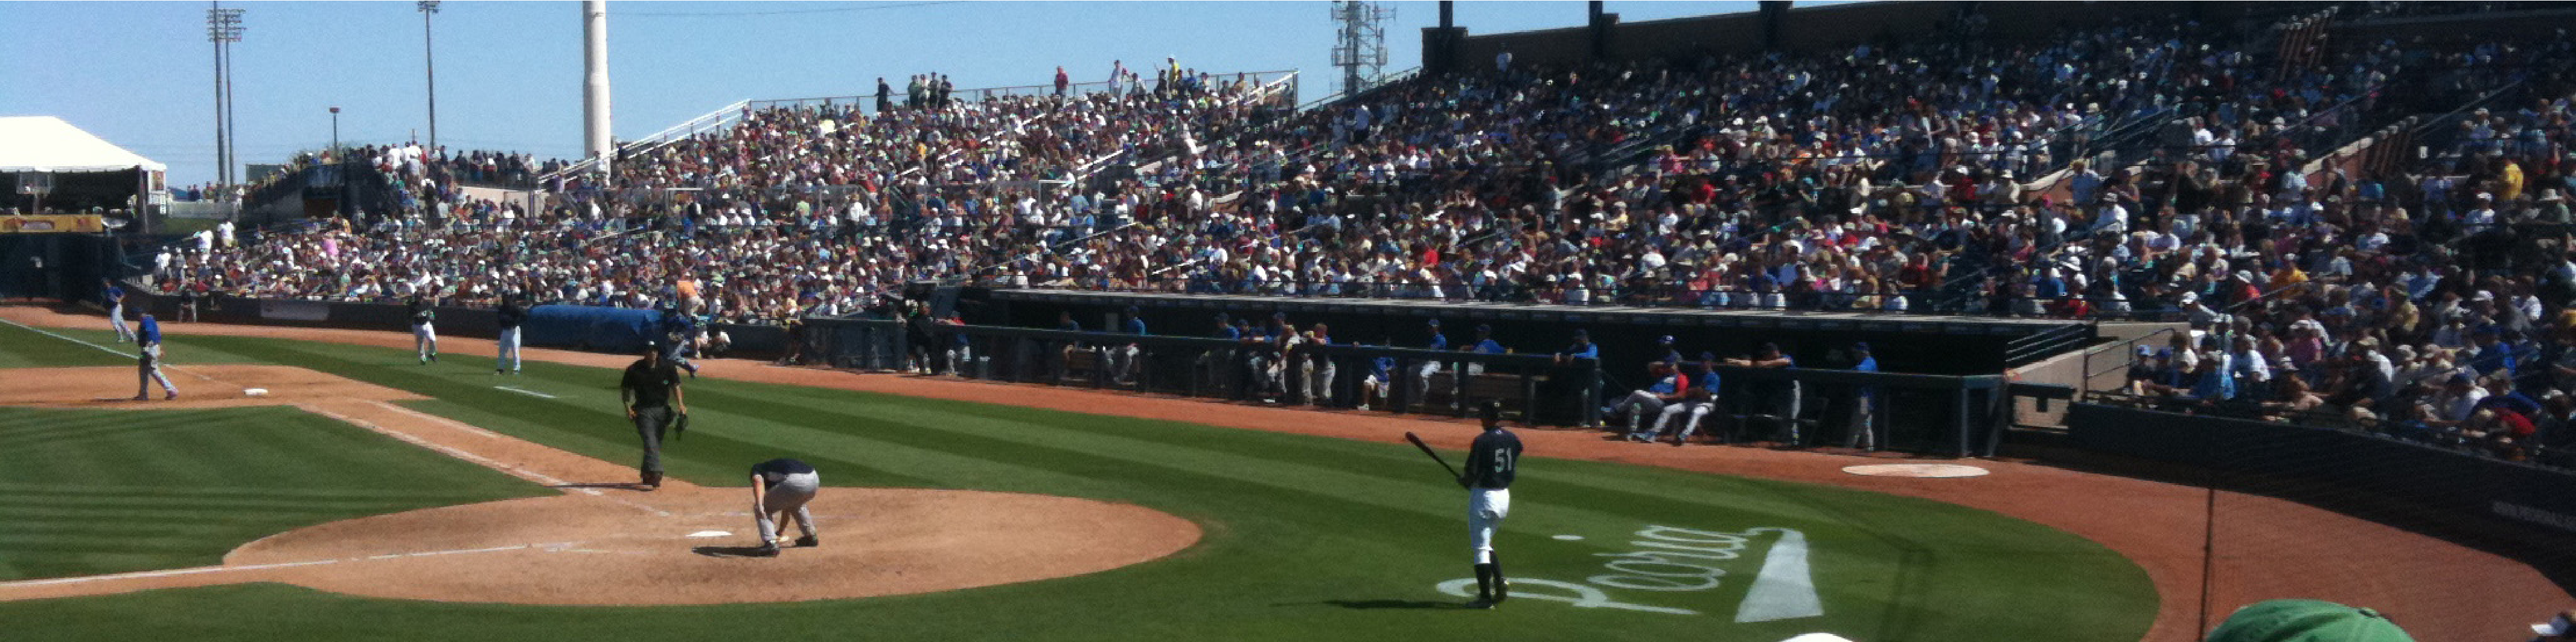
\includegraphics[width=\textwidth]{sampleteaser}
  \caption{Seattle Mariners at Spring Training, 2010.}
  \Description{Enjoying the baseball game from the third-base
  seats. Ichiro Suzuki preparing to bat.}
  \label{fig:teaser}
\end{teaserfigure}





\section{Usage Scenario}

We use crescent dataset to discuss how it works. 




\section{Conclusion and Future work}

Authors of any work published by ACM will need to complete a rights
form. Depending on the kind of work, and the rights management choice
made by the author, this may be copyright transfer, permission,
license, or an OA (open access) agreement.

Regardless of the rights management choice, the author will receive a
copy of the completed rights form once it has been submitted. This
form contains \LaTeX\ commands that must be copied into the source
document. When the document source is compiled, these commands and
their parameters add formatted text to several areas of the final
document:



%% The acknowledgments section is defined using the "acks" environment
%% (and NOT an unnumbered section). This ensures the proper
%% identification of the section in the article metadata, and the
%% consistent spelling of the heading.
\begin{acks}
SHREC, NSF
\end{acks}

%%
%% The next two lines define the bibliography style to be used, and
%% the bibliography file.
\bibliographystyle{ACM-Reference-Format}
\bibliography{sample-base}

%%
%% If your work has an appendix, this is the place to put it.
\appendix

\section{Ablation Experiments}

\subsection{Attention Head And Representation Based SI}

Lorem ipsum dolor sit amet, consectetur adipiscing elit. Morbi
malesuada, quam in pulvinar varius, metus nunc fermentum urna, id
sollicitudin purus odio sit amet enim. Aliquam ullamcorper eu ipsum
vel mollis. Curabitur quis dictum nisl. Phasellus vel semper risus, et
lacinia dolor. Integer ultricies commodo sem nec semper.

\subsection{Part Two}

Etiam commodo feugiat nisl pulvinar pellentesque. Etiam auctor sodales
ligula, non varius nibh pulvinar semper. Suspendisse nec lectus non
ipsum convallis congue hendrerit vitae sapien. Donec at laoreet
eros. Vivamus non purus placerat, scelerisque diam eu, cursus
ante. Etiam aliquam tortor auctor efficitur mattis.

\section{Case Study}

Nam id fermentum dui. Suspendisse sagittis tortor a nulla mollis, in
pulvinar ex pretium. Sed interdum orci quis metus euismod, et sagittis
enim maximus. Vestibulum gravida massa ut felis suscipit
congue. Quisque mattis elit a risus ultrices commodo venenatis eget
dui. Etiam sagittis eleifend elementum.

Nam interdum magna at lectus dignissim, ac dignissim lorem
rhoncus. Maecenas eu arcu ac neque placerat aliquam. Nunc pulvinar
massa et mattis lacinia.

\end{document}
\endinput
%%
%% End of file `sample-authordraft.tex'.
